\subsection{Motivation}


\subsubsection{Einleitung}

Die Workshopteilnehmer sollten zu Beginn für das Thema Affective Computing motiviert werden. Dafür gibt es einen kurze Beschreibung der Emotionen mit den Charakteristiken, wie zum Beispiel, dass Emotionen sehr schnell auftreten, aber dafür ebenfalls sehr ungenau sind. Die Intensität ist ebenfalls ein Merkmale der Emotionen. Eine hohe Intensität ist kurzzeitig und stark im Gegensatz zu einem niedrigen Intensiätsempfinden der Emotionen. Eine geringe Intensität ist dauert länger an und wird auch als Stimmung bezeichnet. 

\subsubsection{Workshop Aufgabe}\label{Workshop Aufgabe}



Ziel der Aufgabe ist es den verschiedenen Benutzerempfindlichkeiten aufzuzeigen. Die Aufgabe soll in zwei Gruppen erfolgen, bei der die Gruppen jeweils verschiedene Websiten angezeigt bekommen haben. Auf der Website sollten diese nach Informationen suchen, um den veröffentlichten Fragebogen auszufüllen. Anschlißend sollten die Emotionen eingetragen werden. Während Gruppe 1 ihre Informationen in Wikipedia recherchierte, durfte Gruppe 2 eine Website besuchen, welche den Inhalt grafisch ergänzt. Dabei zeigte sich folgende Auswertungen der Emotionen, welche in Abbildung 1 und Abbildung 2 dargestellt.

\begin{figure}[!h]
	\centering
	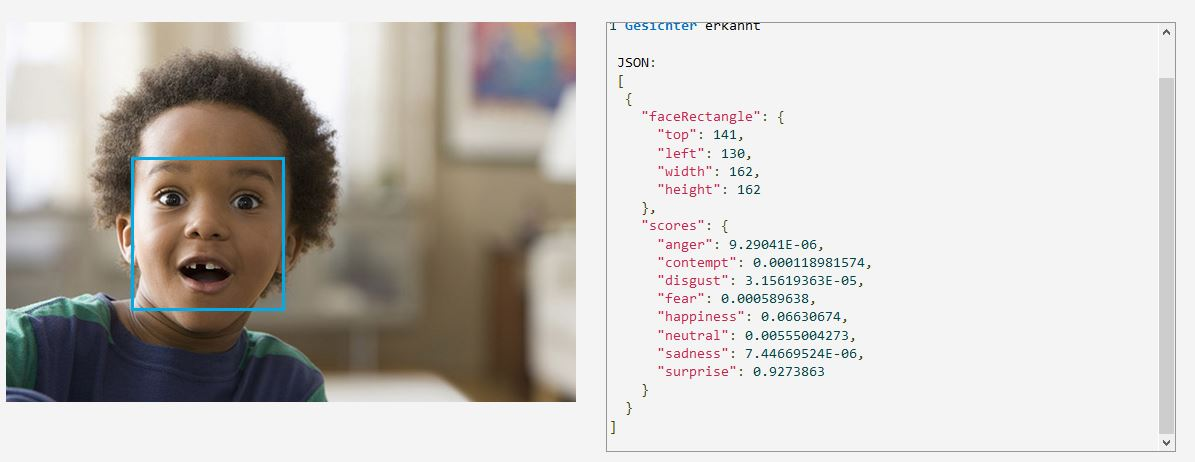
\includegraphics[width=0.9\linewidth]{Pictures/Microsoft_Gestenerkennung}
	\caption[Beispiel: Microsoft Azure Emotionserkennung]{Beispiel: Microsoft Azure Emotionserkennung \cite{MicrosoftAzure}}
	\label{fig:microsoftgestenerkennung}
\end{figure}
